% CVPR 2026 Paper Template; see https://github.com/cvpr-org/author-kit

\documentclass[10pt,twocolumn,letterpaper]{article}

%%%%%%%%% PAPER TYPE  - PLEASE UPDATE FOR FINAL VERSION
% \usepackage{cvpr}              % To produce the CAMERA-READY version
% \usepackage[review]{cvpr}      % To produce the REVIEW version
\usepackage[pagenumbers]{cvpr} % To force page numbers, e.g. for an arXiv version

% Import additional packages in the preamble file, before hyperref
%% This file contains a number of tweaks that are typically applied to the main document.
%% They are not enabled by default, but can be enabled by uncommenting the relevant lines.

%%
%% Inline annotations; for predefined colors, refer to "dvipsnames" in the xcolor package:
%% https://tinyurl.com/overleaf-colors
%%
\newcommand{\red}[1]{{\color{red}#1}}
\newcommand{\todo}[1]{{\color{red}#1}}
\newcommand{\TODO}[1]{\textbf{\color{red}[TODO: #1]}}
%%
%% disable for camera ready / submission by uncommenting these lines  
%%
% \renewcommand{\TODO}[1]{}
% \renewcommand{\todo}[1]{#1}

%%
%% work harder in optimizing text layout. Typically shrinks text by 1/6 of page, enable
%% it at the very end of the writing process, when you are just above the page limit
%%
\usepackage{microtype}

%%
%% fine-tune paragraph spacing
%%
% \renewcommand{\paragraph}[1]{\vspace{.5em}\noindent\textbf{#1.}}

%%
%% globally adjusts space between figure and caption
%%
\setlength{\abovecaptionskip}{.5em}
\setlength{\textfloatsep}{10pt plus 2pt minus 4pt}
\setlength{\dbltextfloatsep}{10pt plus 2pt minus 4pt}
\setlength{\floatsep}{8pt plus 2pt minus 2pt}


%%
%% Allows "the use of \paper to refer to the project name"
%% with automatic management of space at the end of the word
%%
% \usepackage{xspace}
% \newcommand{\paper}{ProjectName\xspace}

%%
%% Commonly used math definitions
%%
% \DeclareMathOperator*{\argmin}{arg\,min}
% \DeclareMathOperator*{\argmax}{arg\,max}

%%
%% Tigthen underline
%%
% \usepackage{soul}
% \setuldepth{foobar}
\usepackage{tikz}
\usetikzlibrary{positioning,arrows.meta}
\usepackage{adjustbox}

% It is strongly recommended to use hyperref, especially for the review version.
% hyperref with option pagebackref eases the reviewers' job.
% Please disable hyperref *only* if you encounter grave issues, 
% e.g. with the file validation for the camera-ready version.
%
% If you comment hyperref and then uncomment it, you should delete *.aux before re-running LaTeX.
% (Or just hit 'q' on the first LaTeX run, let it finish, and you should be clear).
\definecolor{cvprblue}{rgb}{0.21,0.49,0.74}
\usepackage[pagebackref,breaklinks,colorlinks,allcolors=cvprblue]{hyperref}

%%%%%%%%% PAPER ID  - PLEASE UPDATE
\def\paperID{*****} % *** Enter the Paper ID here
\def\confName{CVPR}
\def\confYear{2026}

%%%%%%%%% TITLE - PLEASE UPDATE
\title{Smartphone-Only Occlusion Removal for Estimating Healthy Grape Yield in Vineyards}

%%%%%%%%% AUTHORS - PLEASE UPDATE
% \author{First Author\\
% Institution1\\
% Institution1 address\\
% {\tt\small firstauthor@i1.org}
% % For a paper whose authors are all at the same institution,
% % omit the following lines up until the closing ``}''.
% % Additional authors and addresses can be added with ``\and'',
% % just like the second author.
% % To save space, use either the email address or home page, not both
% \and
% Second Author\\
% Institution2\\
% First line of institution2 address\\
% {\tt\small secondauthor@i2.org}
% }
\author{
Has Salvesen \qquad Finn Panko-Jones \qquad Dinh Quang Huynh\\
{\tt\small \{hsal9391,fpan2183,dhuy9648\}@uni.sydney.edu.au}
}

\begin{document}
\maketitle
\begin{abstract}
Estimating grape crop before harvest still relies largely on sparse, destructive hand sampling, and cameras only help if they can see the fruit. In vineyards, leaves hide much of it from any single view. Robotic harvesters handle occlusion with active perception, moving a camera to a better viewpoint for each fruit. A vehicle driving down a straight vine row cannot do this, but it already supplies a dense sweep of lateral viewpoints as a by-product of its motion. We ask whether that passive sweep, captured by one ordinary RGB camera, can recover hidden fruit well enough to improve a downstream task: counting grapes. Our pipeline segments fruit and foliage with SAM~3, registers views using SIFT features found only on fruit, solves one similarity transform per view jointly with held-out validation, and composites only fruit colours that agree across several views spanning a minimum baseline. It never synthesises unseen fruit. Using a phone on a laboratory rail as a surrogate for a vehicle, we vary viewpoint spacing (20--60~mm) and occlusion (3--6 foreground branches). We evaluate in two ways: pixel-wise against a leaf-free photograph, and by count, using GrapeSAM, a point model trained on the ViViD-5K vineyard dataset and left untuned on our data, against 25 hand-labelled grapes. At 20~mm spacing with five branches, fruit pixel recall rose from 42\% to 87\% and count F1 from 0.42 to 0.77. Benefits fell as sampling became sparser and occlusion heavier. At six branches, recovery was partial (25\% to 42\% recall), and at 60~mm it fell below the single view. All conditions share one physical scene, so this is a controlled proof of concept, not an estimate of field accuracy or yield.
\end{abstract}    
\section{Introduction}
Vineyard yield estimates guide decisions on labour, logistics and crop thinning, yet they are still commonly made by destructive hand sampling, which is labour intensive and too sparse to capture variation across a block~\cite{nuske2014}. A camera carried along the rows could sample every vine. The most accessible version is a smartphone fixed to a vehicle that already drives the rows, such as a tractor or utility vehicle. It needs no depth sensor, LiDAR or multi-camera rig.

The obstacle is occlusion. Leaves, shoots and neighbouring bunches hide fruit, so even a perfect single-image detector undercounts. Hemming \etal~\cite{hemming2014} showed how much viewpoint matters: for sweet pepper, no single camera position detected more than 69\% of fruit, while five positions together reached 90\%. Occlusion is therefore not only a detector problem but a sampling problem. The question is which views to collect and how to combine them.

Harvesting robotics answers this with \emph{active perception}. A manipulator moves the camera to a new viewpoint for each fruit, by next-best-view planning or visual servoing, until the fruit is visible~\cite{magalhaes2022,burusa2024}. This suits a robot that must reach individual fruit, but it needs an arm, per-target planning and time at each plant. Vineyard monitoring is different. Vines are grown in straight trellised rows, and the vehicle's path is fixed by the row. The camera cannot choose its viewpoint. Instead, as the vehicle moves, it passively gathers a dense, ordered sweep of lateral views, in which the near foliage shifts more than the fruit behind it because of parallax. Existing vehicle-based vineyard systems use such sequences mainly to count visible fruit and then correct for hidden fruit statistically~\cite{nuske2014,millan2018}, to avoid double counting across frames~\cite{santos2020,liu2019}, or to predict hidden berries with learned models~\cite{quinones2025gcnet,kierdorf2022}. Tracking-based counters~\cite{liu2019,santos2020,stein2016} credit a fruit that is detected whole in some view, and FruitNeRF~\cite{meyer2024fruitnerf} counts fruit in a radiance field built from many posed views. As far as we know, none composes the partial observations of the sweep into a single de-occluded view of the fruit, so fruit never fully exposed in any one view stays uncounted.

We address that gap. Given a sequence from one moving RGB camera, our pipeline recovers grape pixels hidden in a reference view, using only colours observed in other views. Because it is purely image based, it needs no depth sensor or calibrated poses: alignment is estimated from fruit features in the images themselves, and the only motion input is the nominal view spacing used by a baseline rule that was inactive at the spacings tested (Sec.~\ref{sec:ablation}). As a controlled first step, we use a phone on a horizontal rail as a surrogate for vehicle motion.

Our contributions are (i) a fruit-only registration and observation-backed fusion pipeline: it segments fruit and foliage with SAM~3~\cite{carion2025}, aligns views on fruit features with a jointly solved and validated similarity model, and keeps a pixel only when several views spanning a minimum baseline agree on its colour; (ii) an evaluation that judges recovery by a downstream task as well as by pixels, applying an independently trained grape counter, GrapeSAM~\cite{tong2026vivid}, unchanged to the occluded view, the reconstruction and a leaf-free photograph; and (iii) a controlled study of viewpoint spacing (20--60~mm) and occlusion (3--6 foreground branches), including where and why recovery fails.
We also briefly explore separating red and green fruit, a step toward the ripe and unripe estimate that the title names. This report evaluates the occlusion-removal step only; it does not estimate yield, fruit mass, ripeness or vine health.

\section{Related Work}
\subsection{Occlusion in fruit perception: active versus passive viewpoints}
Occlusion is a long-standing bottleneck for agricultural robots. Bac \etal~\cite{bac2014} reviewed 50 harvesting robots and found average fruit localisation success of 85\% and harvest success of 66\%, and that performance had not improved over three decades. Occlusion was a frequent cause of failure. The dominant response has been active perception. In a systematic review of active perception for fruit harvesting, Magalhães \etal~\cite{magalhaes2022} screened 1,034 publications, kept 195, and found multiple-viewpoint strategies and visual servoing to be the most common, though not yet robust. Recent work plans the next best view of a manipulator-mounted camera to reveal task-relevant plant parts in occluded greenhouse crops~\cite{burusa2024}. Hemming \etal~\cite{hemming2014} quantified why this helps: combining camera positions raised sweet pepper detectability from at most 69\% to 90\%. All of these approaches choose a viewpoint per target, which assumes a manipulator and time spent at each fruit; a vehicle on a straight vine row cannot, and must use the views its motion happens to supply.

\subsection{Vineyard yield estimation and hidden fruit}
Nuske \etal~\cite{nuske2014} mounted a side-facing camera with flash illumination on a vehicle, detected berries in each image and calibrated counts to harvest yield over several seasons. Their estimates explained up to 75\% of spatial yield variance, with an average error of 3--11\% of total yield. Santos \etal~\cite{santos2020} segmented grape clusters with Mask R-CNN and associated detections across video frames in 3D to avoid double counting. Liu \etal~\cite{liu2019} counted orchard fruit with a single camera, tracking detections and building a semantic structure-from-motion map, and matched a system that used LiDAR and GPS/INS. These systems count what is visible and treat occlusion as a bias to correct afterwards.

Several methods model the hidden fruit directly. Millan \etal~\cite{millan2018} used a Boolean model to compensate statistically for partly occluded berries, obtaining $R^2=0.78$ for on-the-go yield on three vine segments. GCNet~\cite{quinones2025gcnet} is the closest to our setting. It images grape clusters indoors against white or simulated backgrounds with artificial foliage, segments them with a U-Net, and adds a regressed correction factor for occluded berries when estimating count and weight. Kierdorf \etal~\cite{kierdorf2022} go further and use a conditional GAN to generate a plausible view of berries behind leaves, which brought counts closer to manual references. These methods estimate hidden fruit from priors learned on other bunches. The result can be accurate on average, but for any given vine the hidden berries are inferred, not observed. Our method takes the opposite position: it recovers only fruit that some other view has actually seen, and leaves the rest empty. A learned correction could then be applied to a smaller remaining gap.

For berry-level counting, ViViD-5K~\cite{tong2026vivid} provides 5,000 vineyard images with over 648,000 berry centroids across 13 varieties, together with GrapeSAM, a point localiser followed by SAM. It reports a counting MAE of 21.46 berries per image on images averaging about 130 berries. We use its published point model unchanged as an independent counter. Its authors note weaker performance on indoor and uniform backgrounds, which applies to our scenes.

\subsection{Seeing through occluders with multiple views}
Synthetic aperture imaging aligns images from many camera positions on a chosen depth, so occluders off that plane blur away. Vaish \etal~\cite{vaish2006} compared focus, stereo and robust statistics such as per-pixel medians for reconstructing surfaces behind foliage. Airborne optical sectioning applies the same principle from a drone to reveal the ground through forest canopy~\cite{kurmi2018}. Each of these requires the target depth or a calibrated camera pose. Obstruction-free photography~\cite{xue2015} removes fences and reflections from a short handheld sequence by separating layers by their motion, and Liu \etal~\cite{liu2020obstruct} learn the same layer separation with optical flow and a CNN. DeOccNet~\cite{wang2020} learns occlusion removal from light fields. Learned methods produce visually complete images, but they inpaint regions no view has seen, which is undesirable when the output is to be counted. Our pipeline sits between these: like obstruction removal, it needs no depth or calibrated poses, but like robust synthetic aperture methods, it never synthesises content that no view observed. Pixel labelling of occluders~\cite{pei2013} and all-in-focus synthetic aperture~\cite{yang2014} are the published remedies for the occluder leakage and multi-depth blur of plain averaging (Sec.~\ref{sec:evolution}). We build on SIFT~\cite{lowe2004}, RANSAC~\cite{fischler1981} and SAM~3~\cite{carion2025}; Sec.~\ref{sec:method} gives the details.

\section{Method}\label{sec:method}
Figure~\ref{fig:pipeline} summarises the pipeline. Given $N$ RGB views $I_1,\ldots,I_N$ from one camera translating along a row, we produce a fruit-only image in the frame of a reference view $r$. Every pixel in it is copied from a view that actually observed fruit there. The pipeline has three stages: segmentation (Sec.~\ref{sec:masks}), fruit-only registration (Sec.~\ref{sec:registration}) and observation-backed fusion (Sec.~\ref{sec:fusion}). Section~\ref{sec:evolution} explains how this design replaced an earlier depth-based prototype.

\begin{figure*}[t]
\centering
\resizebox{\textwidth}{!}{%
\begin{tikzpicture}[
  font=\footnotesize,
  >={Stealth[length=2mm]},
  box/.style={draw, rounded corners=2pt, align=center, text width=3.15cm, minimum height=1.55cm, inner sep=3pt},
  seg/.style={box, fill=green!8},
  reg/.style={box, fill=blue!7},
  fus/.style={box, fill=orange!10},
  io/.style={box, fill=gray!10},
  ev/.style={box, fill=white, dashed},
  arr/.style={->, thick},
  lab/.style={font=\scriptsize\bfseries, text=black!65}
]
% Row 1
\node[io]  (in)   {\textbf{Image sequence}\\ $N$ RGB views, one camera\\ rail (lab) or vehicle (field)};
\node[seg, right=0.55cm of in] (mask) {\textbf{Segmentation}\\ SAM~3 fruit masks $C_i$\\ foliage masks $F_i$\\ \textit{(colour rule: ablation)}};
\node[reg, right=0.55cm of mask] (sift) {\textbf{Fruit-only features}\\ SIFT on $C_i\wedge\neg F_i$\\ 4 neighbours, reciprocal\\ ratio test 0.78};
\node[reg, right=0.55cm of sift] (pair) {\textbf{Pairwise RANSAC}\\ similarity, $\tau_g{=}1.5$\,px\\ fit on $\tfrac34$, hold out $\tfrac14$\\ scale, rotation gates};
% Row 2
\node[reg, below=0.75cm of pair] (graph) {\textbf{View graph}\\ accepted pairs as edges\\ reference $r$ = best\\ connected view};
\node[reg, left=0.55cm of graph] (solve) {\textbf{Joint pose solve}\\ IRLS, $\mathcal{T}_r=\mathbf{I}$\\ drop view if held-out\\ median error $>3$\,px};
\node[fus, left=0.55cm of solve] (fuse) {\textbf{Consensus fusion}\\ warp to $r$; median colour\\ RMS $\le 30$, $\ge 3$ views\\ span $\ge 40$\,mm};
\node[io, left=0.55cm of fuse] (out) {\textbf{Fruit-only image}\\ colour copied from one\\ observing view; unseen\\ pixels left empty};
% Row 3: evaluation
\node[ev, below=0.75cm of out] (pix) {\textbf{Pixel evaluation}\\ recall, precision, IoU\\ vs.\ registered\\ leaf-free photo};
\node[ev, right=0.55cm of pix] (cnt) {\textbf{Count evaluation}\\ GrapeSAM (untuned) on\\ occluded, restored and\\ leaf-free images};
% Arrows
\draw[arr] (in) -- (mask);
\draw[arr] (mask) -- (sift);
\draw[arr] (sift) -- (pair);
\draw[arr] (pair) -- (graph);
\draw[arr] (graph) -- (solve);
\draw[arr] (solve) -- (fuse);
\draw[arr] (fuse) -- (out);
\draw[arr, dashed] (out.south) -- (pix.north);
\draw[arr, dashed] ([yshift=-0.37cm]out.south) -| (cnt.north);
\draw[arr, densely dotted] (mask.south) to[bend right=12] node[lab, pos=0.55, left] {masks} (fuse.north);
% Stage labels
\node[lab, above=1pt of mask.north] {SEGMENTATION};
\node[lab, above=1pt of sift.north east] {REGISTRATION};
\node[lab, below=1pt of pix.south east] {EVALUATION};
\node[lab, below=1pt of fuse.south east] {FUSION};
\end{tikzpicture}}
\caption{Pipeline overview. Fruit and foliage masks restrict feature matching to fruit, so that the occluding layer, which moves differently under parallax, does not drive the alignment. Pairwise similarities are combined in a view graph and solved jointly, and views failing held-out validation are dropped. Fusion keeps a pixel only when enough views, spanning enough baseline, agree on its colour, then copies that colour from one observing view. Dashed boxes are the evaluation (Sec.~\ref{sec:exp}), not part of the method.}
\label{fig:pipeline}
\end{figure*}

\subsection{Acquisition and assumptions}\label{sec:capture}
The intended field system is a side-facing smartphone on a vehicle that drives along a vine row, recording overlapping views of the canopy. To isolate the vision problem, we reproduce this motion indoors. A phone translates horizontally on a rigid rail past a scene of red grapes on branches, with removable foreground foliage in front (Fig.~\ref{fig:setup}). Illumination is held approximately constant during a sequence. The rail positions are used only to define experimental spacings and the baseline rule in Eq.~\eqref{eq:fusion}. Alignment itself is estimated from the images.

We assume that (i) the camera mainly translates parallel to the row with little rotation, (ii) the fruit layer is approximately planar, so a 2D similarity transform aligns it between nearby views, (iii) the scene is static during capture, and (iv) the foliage lies in front of the fruit, so parallax exposes different parts of the fruit in different views. Assumptions (i) and (iii) match a slow vehicle on a straight row better than handheld capture. Assumption (ii) is the weakest for deep clusters and is examined in Sec.~\ref{sec:exp}.

\begin{figure}[t]
 \centering
 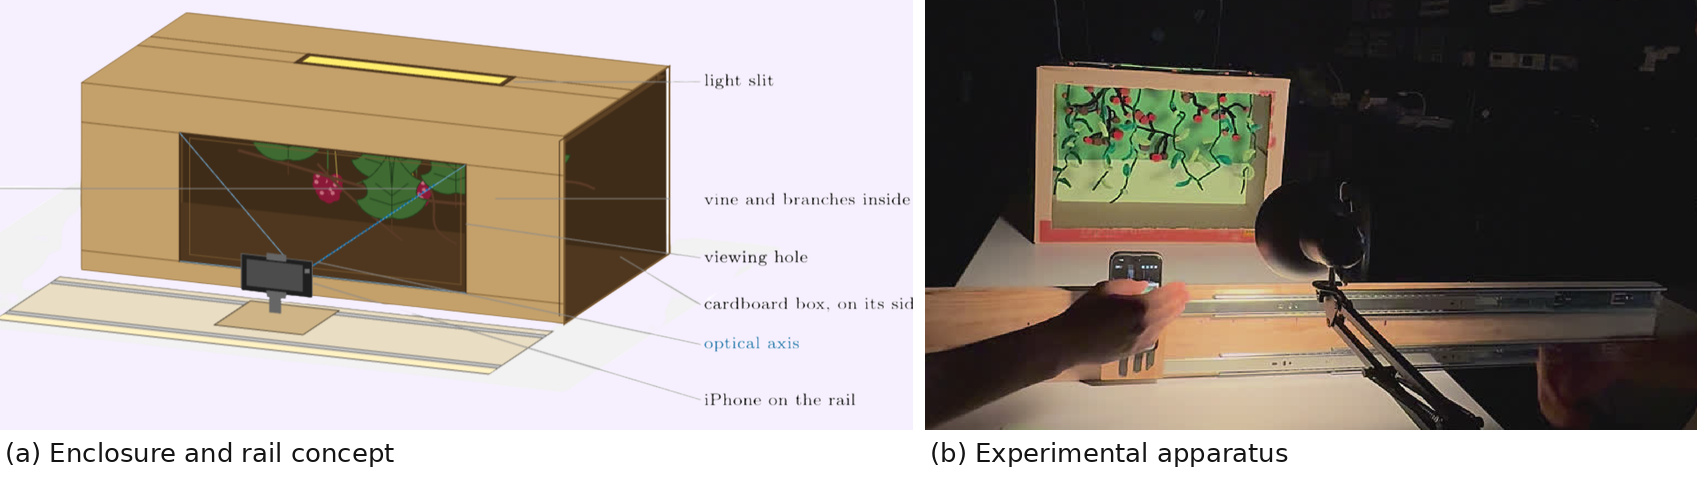
\includegraphics[width=0.86\linewidth]{figures/capture_setup.png}
 \caption{Capture rig: (a) enclosure with a horizontal camera rail and separated fruit and foliage layers, and (b) the phone, rail, lighting and scene. The rail stands in for vehicle motion along a row.}
 \label{fig:setup}
\end{figure}

\subsection{Fruit and foliage segmentation}\label{sec:masks}
For each view, we obtain a binary fruit mask $C_i(\mathbf{x})$ and a foliage mask $F_i(\mathbf{x})$ from SAM~3 text prompts~\cite{carion2025}: ``grape'' for fruit, and ``green leaf'', ``green vine'' and ``green stem'' for foliage, with fruit taking precedence where the two overlap. A pixel is usable fruit evidence when $E_i(\mathbf{x}) = C_i(\mathbf{x})\,\big(1-F_i(\mathbf{x})\big) = 1$. Excluding foliage matters at fruit boundaries, where a mask may extend over an overlapping leaf. As an ablation, we replace $C_i$ with fixed colour thresholds within a fixed region of interest. This works for red fruit against green leaves, but fails for green fruit: a green rule tuned on two captures reached only 0.31 IoU against SAM~3 masks on a held-out capture. We do not validate SAM~3's masks independently. Because the truth masks used for evaluation also come from SAM~3, the pixel-wise evaluation is not independent of this stage. On mixed red and green scenes we also split the SAM~3 fruit masks with a colour ratio rule, a qualitative step towards the ripe and unripe estimate that we do not evaluate here.

\subsection{Fruit-only registration}\label{sec:registration}
\textbf{Pairwise matching.} SIFT keypoints~\cite{lowe2004} are detected only inside the usable fruit region $E_i$. Restricting features to fruit is the key design choice. Foliage is closer to the camera and so moves further between views, and it often carries more texture, so whole-image matching would align the occluder rather than the target. Each view is matched to its next four neighbours, keeping reciprocal nearest neighbours that pass a 0.78 ratio test. A quarter of the matches are held out. A similarity transform $\mathcal{T}_{ij}$ (scale, rotation and translation) is fitted to the rest with RANSAC~\cite{fischler1981}, counting a correspondence as an inlier when
\begin{equation}
 \left\|\mathbf{p}_j - \mathcal{T}_{ij}(\mathbf{p}_i)\right\|_2 < \tau_g, \qquad \tau_g = 1.5~\text{px}.
 \label{eq:ransac}
\end{equation}
A pair is accepted only if it has at least 12 inliers and an inlier ratio of at least 0.5, if at least half of the held-out matches transfer within $2\tau_g$, and if its scale lies within 6\% of unity and its rotation within $3^\circ$. These gates follow from assumption (i). They reject pairs matched between similar-looking berries, which repeated texture makes common.

\textbf{View graph and reference.} Accepted pairs form edges of a graph over views. Only views connected to the reference can contribute. The reference is chosen automatically from the largest connected group: the view with the most accepted edges, then the most inliers, then the one closest to the group centre. If the joint solve below fails for that view, the next candidate is tried.

\textbf{Joint pose solve.} Chaining pairwise transforms accumulates drift, so we solve for one similarity $\mathcal{T}_i$ per view jointly, with $\mathcal{T}_r$ fixed to the identity:
\begin{equation}
 \min_{\{\mathcal{T}_i\}} \sum_{(i,j)\in\mathcal{E}} \sum_{k}
 w_{ijk}\,\big\|\mathcal{T}_i(\mathbf{p}^{i}_k) - \mathcal{T}_j(\mathbf{p}^{j}_k)\big\|_2^2 .
 \label{eq:joint}
\end{equation}
The problem is linear in the similarity parameters. We solve it by iteratively reweighted least squares over six iterations, with $w_{ijk}=n_{ij}^{-1}\min(1,\tau_g/e_{ijk})$. Here $e_{ijk}$ is the current residual, and $n_{ij}\le 80$ is the number of correspondences sampled from edge $(i,j)$, so that no single feature-rich pair dominates. The held-out matches are then transferred through the solved poses. Any view whose median held-out error exceeds 3~px is removed, together with its edges. A reconstruction is attempted only if at least three views remain. With SAM~3 masks at 20~mm spacing, 84--95 of 102 tested pairs passed for three to five branches, but only 40 of 98 at six branches, where 13 views were removed. More views therefore do not guarantee a larger usable aperture.

\subsection{Observation-backed fusion}\label{sec:fusion}
Each view and its masks are warped into the reference frame, $\tilde I_i(\mathbf{x}) = I_i(\mathcal{T}_i^{-1}(\mathbf{x}))$, and similarly for $\tilde E_i$. Let $\tilde V_i(\mathbf{x})$ indicate that the pixel lies inside view $i$, so that candidate observations are those with $\tilde E_i \tilde V_i = 1$. At each pixel, we take the per-channel median colour $\boldsymbol{\mu}(\mathbf{x})$ of the candidates and keep the agreeing set
\begin{equation}
 \mathcal{A}(\mathbf{x}) = \big\{\, i : \tilde E_i\tilde V_i = 1,\ d_i(\mathbf{x}) \le \tau_c \,\big\},
 \label{eq:agree}
\end{equation}
where $d_i$ is the RMS RGB distance of $\tilde I_i(\mathbf{x})$ from $\boldsymbol{\mu}(\mathbf{x})$ and $\tau_c=30$. The pixel is output as fruit when
\begin{equation}
 \hat G(\mathbf{x}) = \mathbf{1}\big[\,|\mathcal{A}(\mathbf{x})| \ge m\,\big]\;
 \mathbf{1}\big[\,B(\mathbf{x}) \ge B_{\min}\,\big],
 \label{eq:fusion}
\end{equation}
with $m=3$ views. $B(\mathbf{x})$ is the rail distance between the outermost agreeing views, and $B_{\min}=40$~mm. The median rejects a minority of misaligned or mis-segmented observations. The baseline condition requires that agreement comes from genuinely different viewpoints, not from neighbouring views that share the same occlusion.

The output colour is copied from a single agreeing view, not blended, so no colour is synthesised. The view is chosen to minimise a cost. The cost combines its smoothed colour deviation $d_i/\tau_c$, a small penalty near the boundary of its agreeing region, and a slight preference for views near the reference. This reduces visible seams between sources. Pixels with $\hat G=0$ are left empty, and fruit regions smaller than 25~px are removed. The output thus distinguishes recovered fruit from fruit that was never observed. An empty region means unobserved, not absent.

\subsection{Design evolution}\label{sec:evolution}
Our first prototype used depth-based synthetic aperture imaging~\cite{vaish2006}. For a camera translated by $B_i$ parallel to the image plane, a point at depth $Z_t$ shifts by $\Delta u_i \simeq f_x B_i / Z_t$ pixels. Shifting each view by this amount aligns the fruit plane, and the occluders, at a different depth, are blurred out by a per-pixel median or a masked mean (Fig.~\ref{fig:sai}). This required the fruit depth and the camera step to be known, and errors grow with baseline, as $\delta(\Delta u) \simeq -(f_x B_i / Z_t^2)\,\delta Z_t$. Fruit at several depths blurred, residual foliage remained, and the output was an image rather than a fruit segmentation. Replacing known geometry with fruit-only feature registration removed the need for depth and step measurements. Replacing averaging with consensus selection removed blur and produced a fruit-only output. A parallel line, a colour-free occlusion-aware synthetic aperture that finds the foliage from multi-view depth rather than colour, was developed alongside and benchmarked only on synthetic scenes; its code and results are in the repository~\cite{teamrepo}, and it is not used for the results below.

\begin{figure}[t]
 \centering
 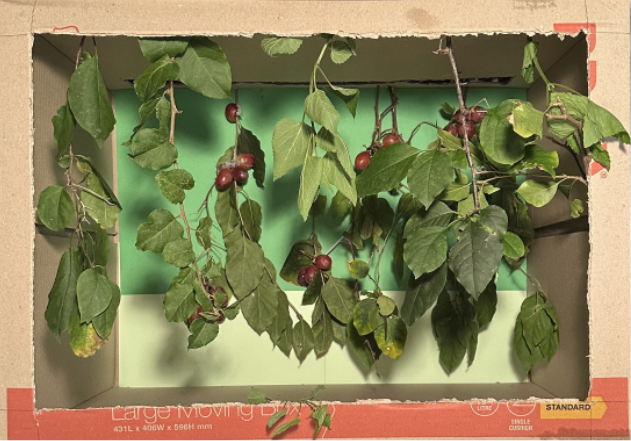
\includegraphics[width=0.44\linewidth]{figures/sai_input.png}\hfill
 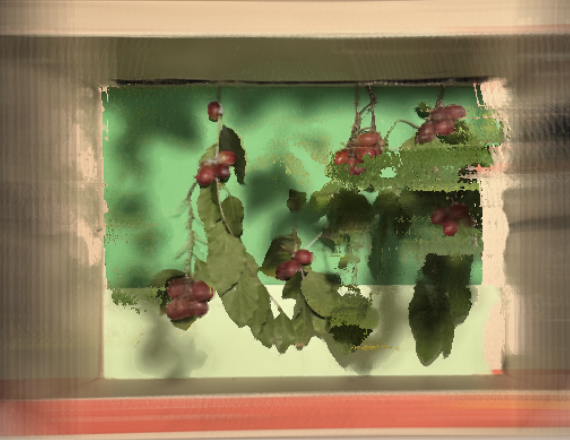
\includegraphics[width=0.44\linewidth]{figures/sai_output.png}
 \caption{Depth-based synthetic aperture prototype: occluded input (left) and fused refocused view (right). Some foliage is suppressed, but much remains, and the output is not a fruit segmentation.}
 \label{fig:sai}
\end{figure}



\section{Experimental Setup}\label{sec:exp}
\subsection{Data and conditions}
We vary \emph{occlusion}, using 3, 4, 5 or 6 foreground branches, and \emph{viewpoint spacing}, using 20, 40 or 60~mm. Each branch count has one rail capture of 28 views at 20~mm steps (27 at six branches). The 40 and 60~mm conditions keep every second or third view around the same reference, so that spacing changes while the scene and reference stay fixed. Images are processed at 0.8 of full resolution ($2419\times3226$~px, width by height; the phone was held in portrait). Fruit and foliage masks come from SAM~3 and were stored with each capture. All conditions share one physical arrangement of red grapes. The study therefore characterises these conditions, not a population of scenes.

\textbf{Ground truth.} After the foliage was removed, a leaf-free photograph of the same fruit was taken from a different position. Its fruit mask comes from SAM~3, and we hand-labelled the centres of its 25 grapes. For each capture, the photograph is registered to the reference view with a similarity transform fitted to SIFT features near the fruit. We inspected an overlay for every branch count. Agreement is good overall, but some clusters at five and six branches show visible offset, because the fruit lies at different depths.

\subsection{Metrics}
\textbf{Pixel-wise.} With registered truth fruit mask $G$ and recovered mask $\hat G$, we report recall $R=|G\cap\hat G|/|G|$, precision $P=|G\cap\hat G|/|\hat G|$ and IoU. The single-view baseline applies the same formulas to the reference view's own fruit mask. Because $G$ also comes from SAM~3, this evaluation shares a model with the method.

\textbf{Count-based.} Pixel overlap cannot tell whether recovered fruit is still separable into berries. We therefore run the GrapeSAM point model~\cite{tong2026vivid}, with its published weights and post-processing (confidence 0.05), on three fruit-only images: the occluded reference view, the reconstruction and the registered leaf-free photograph. None of its settings were tuned on our data. Detections are matched one-to-one to the 25 labels, closest first, within 24~px, which is about one berry radius. We report count F1, the number of detections $n$, and average precision (AP) over a sweep of confidence thresholds. We call the leaf-free result a \emph{comparison point} rather than a ceiling, because GrapeSAM overcounts it (29--40 detections for 25 grapes).

\textbf{Uncertainty.} With one scene, we cannot measure variation between scenes, so we estimate three narrower sources: which grapes happen to be present (2,000 bootstrap resamples of the 25 grapes, paired between the single view and the reconstruction); the choice of reference (the 20~mm runs repeated with four other references, offset by $\pm4$ and $\pm8$ views); and truth registration error (the truth transform perturbed by shifts of 1--5~px in eight directions, rotations of $\pm0.5^\circ$ and $\pm1^\circ$ and scale changes of $\pm1\%$, then all metrics recomputed).

\subsection{Baselines and ablations}
All baselines use the same views, masks and evaluation. \emph{Mask voting} takes the union, or the majority, of the aligned SAM~3 fruit masks, coloured by the median observed fruit colour. \emph{Synthetic aperture} (SA)~\cite{vaish2006} takes the per-pixel mean, median or foliage-masked mean of the aligned stack, then segments the fused image with SAM~3. We test SA under two alignments. \emph{Depth shift}, our prototype (Sec.~\ref{sec:evolution}), applies one horizontal shift per rail step, chosen by maximising focus over the reference fruit region. \emph{Our alignment} uses the jointly solved poses, which isolates the effect of the fusion rule. Component ablations use five branches at 20~mm, where the gain is largest. Fusion and mask variants reuse the full method's poses. Alignment variants re-solve the poses and pass them through the same validation.

To separate spacing from the number of views, we vary the number of views centred on the reference at 20~mm, from 3 to 28. We also fix nine views at 20, 40 and 60~mm, and fix the span at 480~mm, which takes 25, 13 and 9 views at those spacings.

\textbf{Implementation.} The code is in Python with OpenCV~\cite{opencv}, NumPy~\cite{numpy}, Pillow and scikit-image; SAM~3~\cite{sam3code} and GrapeSAM~\cite{tong2026vivid} run under PyTorch~\cite{pytorch} on the GPU. The pipeline, the mask scripts and the scripts that produce the tables and figures are in our code repository~\cite{teamrepo}. As a check of the code, a repeat run on one capture reproduced the same reference view, the same accept or reject decision for 101 of the 102 tested pairs and the same 13,395 observed pixels.

\section{Results}
\subsection{Recovery across occlusion and spacing}
Table~\ref{tab:main} gives every condition. At 20~mm, reconstruction raised fruit pixel recall at every branch count: from 68\% to 94\% with three branches, 49\% to 87\% with four, 42\% to 87\% with five, and 25\% to 42\% with six. It kept precision at 77--82\%. Count F1 rose by a similar margin: 0.62 to 0.79, 0.56 to 0.76, 0.42 to 0.77 and 0.14 to 0.55. At six branches, recovery is only partial. Just 14 of 27 views passed alignment validation, and whole clusters are missing (Fig.~\ref{fig:qual}); the reference view's own mask had 41\% precision there, which consensus raised to 77\%.

Wider spacing helped only under light occlusion. With three branches, 40~mm gave the best count F1 (0.88; its 25 detections hide three misses offset by three false positives, which is why we match detections rather than compare totals). With four or more branches, wider spacing lost recall, and losses track view rejection. At five branches and 40~mm, only 8 of 14 views survived, and both recall and F1 fell to the single-view level. At six branches and 60~mm, 3 of 9 views survived, recall fell below the single view, and GrapeSAM detected nothing.

\begin{table}[t]
\centering
\caption{Main results with SAM~3 masks. Views are those kept after alignment validation. Fruit-pixel recall $R$, precision $P$ and IoU are for the reconstruction, with the occluded reference view's recall as $R_\text{single}$. Count F1 is GrapeSAM against 25 labels, and $n$ is its number of detections on the reconstruction. Single-view precision is 85, 81, 86 and 41\% for 3--6 branches.}
\label{tab:main}
\scriptsize
\setlength{\tabcolsep}{3.6pt}
\begin{tabular}{@{}ccc cccc ccc@{}}
\toprule
 & & & \multicolumn{4}{c}{Fruit pixels (\%)} & \multicolumn{3}{c}{GrapeSAM count}\\
\cmidrule(lr){4-7}\cmidrule(lr){8-10}
Br. & mm & Views & $R_\text{single}$ & $R$ & $P$ & IoU & $F1_\text{single}$ & $F1$ & $n$\\
\midrule
3 & 20 & 28/28 & 68 & 94 & 80 & 0.76 & 0.62 & 0.79 & 36\\
3 & 40 & 14/14 & 68 & 92 & 86 & 0.80 & 0.62 & 0.88 & 25\\
3 & 60 & 9/9 & 68 & 88 & 90 & 0.80 & 0.62 & 0.83 & 23\\
\addlinespace[1pt]
4 & 20 & 28/28 & 49 & 87 & 80 & 0.72 & 0.56 & 0.76 & 30\\
4 & 40 & 14/14 & 49 & 74 & 84 & 0.65 & 0.56 & 0.72 & 22\\
4 & 60 & 7/9 & 49 & 52 & 89 & 0.49 & 0.56 & 0.54 & 12\\
\addlinespace[1pt]
5 & 20 & 28/28 & 42 & 87 & 82 & 0.73 & 0.42 & 0.77 & 27\\
5 & 40 & 8/14 & 42 & 42 & 91 & 0.40 & 0.42 & 0.39 & 6\\
5 & 60 & 9/9 & 42 & 57 & 93 & 0.54 & 0.42 & 0.48 & 8\\
\addlinespace[1pt]
6 & 20 & 14/27 & 25 & 42 & 77 & 0.38 & 0.14 & 0.55 & 15\\
6 & 40 & 8/13 & 25 & 27 & 87 & 0.26 & 0.14 & 0.28 & 4\\
6 & 60 & 3/9 & 25 & 9 & 80 & 0.08 & 0.14 & 0.00 & 0\\
\bottomrule
\end{tabular}
\end{table}

\begin{figure*}[t]
\centering
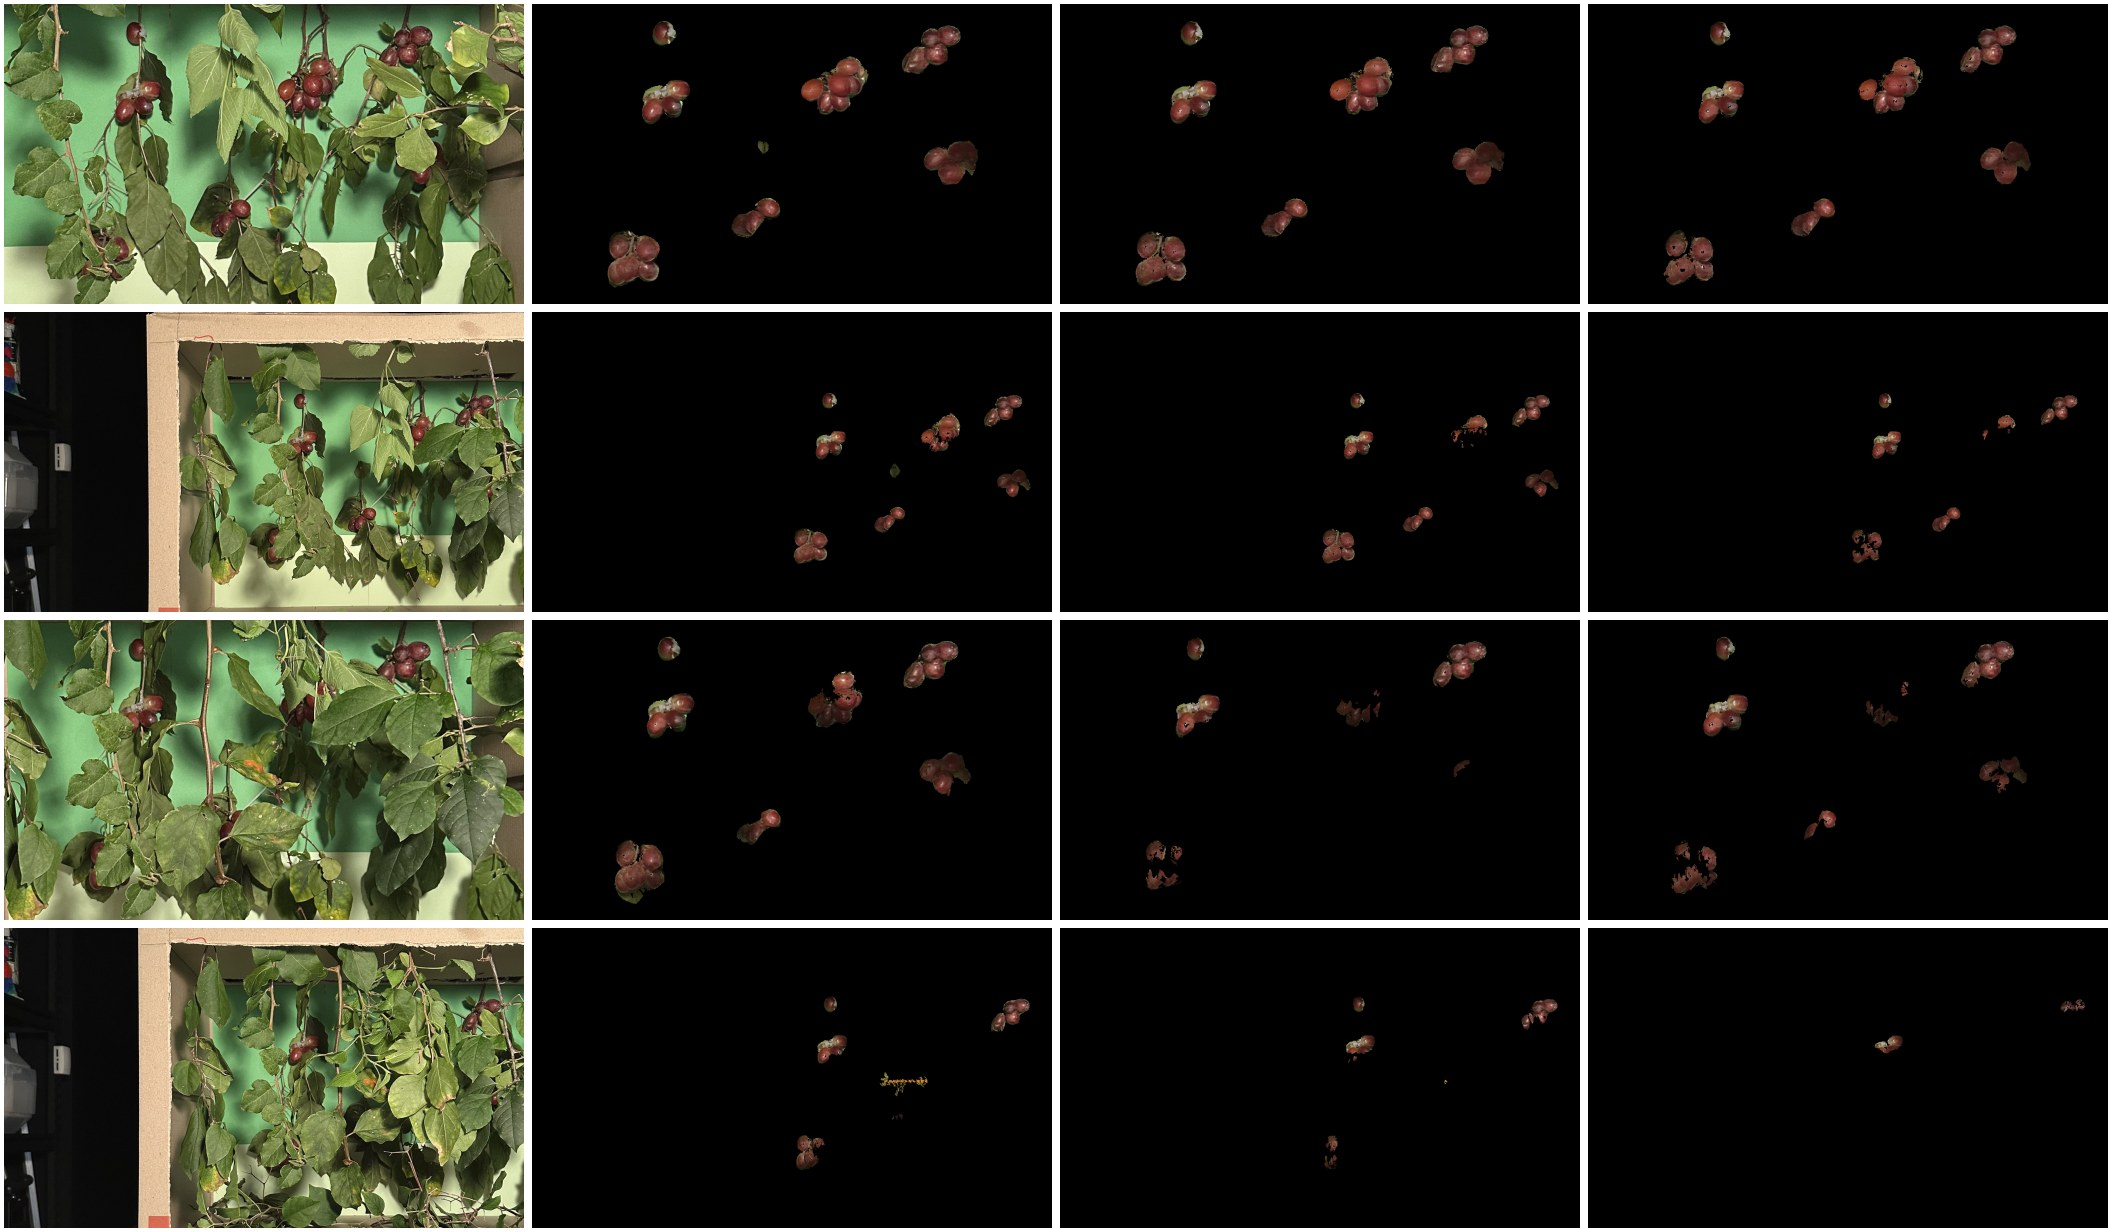
\includegraphics[width=0.42\textwidth]{figures/qualitative_grid.jpg}
\caption{Qualitative results. Rows show 3--6 foreground branches. Columns show the occluded reference view, then reconstructions at 20, 40 and 60~mm spacing, all cropped to the same fruit region. Black means no observation-backed fruit. Clusters disappear as spacing widens under heavy occlusion. At six branches, a strip of stem passed through the masks at 20~mm, and almost nothing survived at 60~mm.}
\label{fig:qual}
\end{figure*}

\subsection{Comparison with baselines}
Table~\ref{tab:baselines} compares fusion rules on the same views. Alignment is the larger factor. Depth-shift synthetic aperture, our prototype, gave count F1 of 0.72 to 0.78 at three branches; the mean and median collapsed to 0.08 at five branches, and all three statistics to 0.00 at six. Switching the same statistics to our feature-based alignment recovered much of the loss for the median (0.54 to 0.68, 0.08 to 0.44 and 0.00 to 0.33 at four to six branches) and the masked mean. The plain mean stayed poor, because foliage still contaminates it. Among the fusion rules, mask union had the highest recall (94--95\% up to five branches) but a precision of only 59--66\%. Mask majority had the opposite profile, with only 22\% recall at five branches. Our consensus rule combined 87\% recall with 80--82\% precision at four and five branches. Every other rule was at least six points lower in recall or in precision. It also had the best or equal-best count F1 at five and six branches. At three branches, the aligned median (0.84) and mask union (0.83) counted slightly better than ours (0.79). At four, the aligned masked mean was level with ours (0.78 against 0.76). These differences are similar in size to the effect of shifting the truth registration by 5~px (up to 0.08 F1), so we do not read them as a ranking.

\begin{table*}[t]
\centering
\caption{Fusion baselines at 20~mm, all using SAM~3 masks and the same views. $R$ and $P$ are fruit-pixel recall and precision (\%), and F1 is the GrapeSAM count F1. SA is synthetic aperture~\cite{vaish2006}. ``Depth shift'' is our prototype's alignment, and ``our alignment'' uses the poses of Sec.~\ref{sec:registration}. SA outputs are segmented by running SAM~3 on the fused image.}
\label{tab:baselines}
\scriptsize
\begin{tabular}{@{}lcccccccccccc@{}}
\toprule
Method & \multicolumn{3}{c}{3 branches} & \multicolumn{3}{c}{4 branches} & \multicolumn{3}{c}{5 branches} & \multicolumn{3}{c}{6 branches}\\
\cmidrule(lr){2-4}\cmidrule(lr){5-7}\cmidrule(lr){8-10}\cmidrule(lr){11-13}
 & R & P & F1 & R & P & F1 & R & P & F1 & R & P & F1\\
\midrule
Single view & 68 & 85 & 0.62 & 49 & 81 & 0.56 & 42 & 86 & 0.42 & 25 & 41 & 0.14\\
\addlinespace[2pt]
Mask union & 95 & 66 & 0.83 & 94 & 59 & 0.76 & 94 & 63 & 0.73 & 60 & 41 & 0.55\\
Mask majority & 75 & 97 & 0.72 & 46 & 95 & 0.48 & 22 & 92 & 0.21 & 14 & 83 & 0.21\\
\addlinespace[2pt]
SA mean, depth shift & 85 & 88 & 0.72 & 76 & 79 & 0.21 & 65 & 83 & 0.08 & 0 & 0 & 0.00\\
SA median, depth shift & 83 & 89 & 0.72 & 71 & 76 & 0.54 & 50 & 88 & 0.08 & 0 & 0 & 0.00\\
SA masked mean, depth shift & 95 & 65 & 0.78 & 95 & 56 & 0.55 & 93 & 60 & 0.50 & 0 & 0 & 0.00\\
\addlinespace[2pt]
SA mean, our alignment & 87 & 87 & 0.56 & 74 & 77 & 0.31 & 80 & 76 & 0.25 & 45 & 73 & 0.00\\
SA median, our alignment & 90 & 85 & 0.84 & 71 & 85 & 0.68 & 53 & 89 & 0.44 & 28 & 73 & 0.33\\
SA masked mean, our alignment & 95 & 76 & 0.79 & 94 & 64 & 0.78 & 89 & 70 & 0.72 & 61 & 65 & 0.41\\
\addlinespace[2pt]
Ours & 94 & 80 & 0.79 & 87 & 80 & 0.76 & 87 & 82 & 0.77 & 42 & 77 & 0.55\\
\bottomrule
\end{tabular}
\end{table*}

\subsection{Ablations}\label{sec:ablation}
Table~\ref{tab:ablation} varies one component at a time at five branches. \textbf{Colour consensus is what keeps the output countable.} Without it, pixel recall and precision barely changed (89\% and 80\%), but count F1 fell from 0.77 to 0.26. Removing every consensus rule gave 94\% recall but an F1 of 0.30. Pixel metrics alone would rate these variants as good as the full method. We attribute the drop, without testing it directly, to colour copied from inconsistent sources breaking up berry appearance.

\textbf{Minimum views} trades recall for precision. Raising $m$ from 1 to 3 raised precision from 63\% to 82\% with no loss in count F1, but $m=5$ cost 10 points of recall and reduced F1 to 0.67. \textbf{The minimum span} had no effect up to 40~mm, because at 20~mm spacing any three distinct views already span 40~mm. The rule matters only for denser sampling, such as video, and 80~mm removed real fruit. Copying versus blending the output colour made no measurable difference.

\textbf{Fruit-only features are essential.} With SIFT on the whole image, fewer than three views passed validation and no reconstruction was produced. Colour masks in place of SAM~3 lost 21 points of recall. The joint solve and held-out check did not matter here, because no view was rejected at five branches. Chained similarities and a translation-only model did equally well, although translation-only raised the median held-out error from 0.68 to 1.04~px. A homography overfitted (F1 0.59), and the foliage mask had no measurable effect.

\begin{table}[t]
\centering
\caption{Ablations at five branches and 20~mm. Fusion and mask variants reuse the full method's poses. Values are fruit-pixel recall and precision (\%) and GrapeSAM count F1.}
\label{tab:ablation}
\scriptsize
\setlength{\tabcolsep}{4pt}
\begin{adjustbox}{max width=\linewidth,center}
\begin{tabular}{@{}llccc@{}}
\toprule
Component & Variant & R & P & F1\\
\midrule
Full method & $m{=}3$, $B_{\min}{=}40$, $\tau_c{=}30$, copy & 87 & 82 & 0.77\\
Min.\ views ($B_{\min}{=}0$) & $m=1$ & 93 & 63 & 0.77\\
 & $m=2$ & 91 & 76 & 0.77\\
 & $m=5$ & 77 & 89 & 0.67\\
Min.\ span ($m{=}3$) & $B_{\min}=0$ or 20~mm & 87 & 82 & 0.77\\
 & $B_{\min}=80$~mm & 82 & 84 & 0.71\\
Colour consensus & $\tau_c=15$ & 83 & 83 & 0.68\\
 & $\tau_c=60$ & 88 & 81 & 0.60\\
 & off & 89 & 80 & 0.26\\
 & no consensus at all & 94 & 63 & 0.30\\
Output colour & median blend & 87 & 82 & 0.76\\
Masks & colour rule for fruit & 66 & 87 & 0.54\\
 & no fruit mask & 87 & 1 & 0.53\\
 & no foliage mask & 87 & 82 & 0.77\\
Alignment & whole-image SIFT & \multicolumn{3}{c}{failed}\\
 & chained similarity & 88 & 82 & 0.81\\
 & chained homography & 71 & 70 & 0.59\\
 & joint translation only & 87 & 82 & 0.77\\
\bottomrule
\end{tabular}
\end{adjustbox}
\end{table}

\subsection{Number of views versus spacing}
Figure~\ref{fig:views} varies the number of 20~mm views around the reference. Recall rose steadily with the number of views, from 33\% to 87\% at four branches and from 24\% to 87\% at five. About seven views were needed to beat the single view on pixels, while count F1 overtook it with five to seven views.

Holding the span fixed at 480~mm (25, 13 and 9 views at 20, 40 and 60~mm) isolates sampling density: four-branch recall was 83, 72 and 52\% (F1 0.77, 0.74 and 0.54), and five-branch recall 85, 42 and 57\%, the 40~mm run keeping only 8 of 13 views. With nine views at each spacing, wider spacing helped only at three branches (F1 0.78, 0.92 and 0.83, against 0.58, 0.44 and 0.48 at five). Within the range tested, recovery depends mainly on how many views pass alignment, not on the baseline.

\begin{figure}[t]
\centering
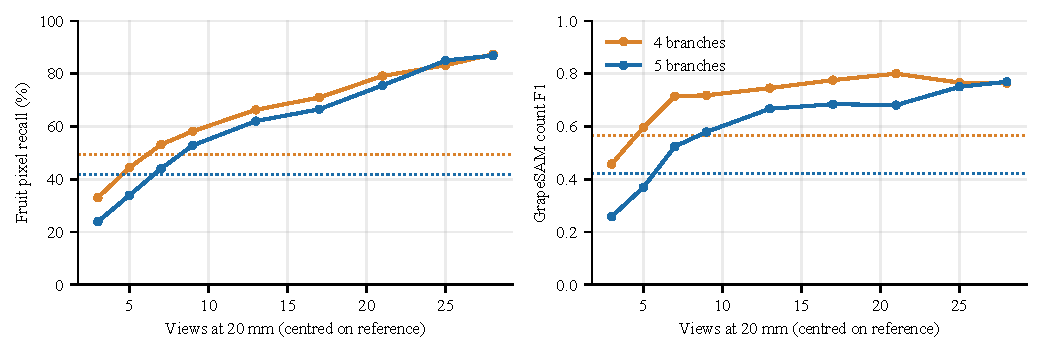
\includegraphics[width=0.9\linewidth]{figures/views_curve.pdf}
\caption{Recall (left) and count F1 (right) against the number of 20~mm views centred on the reference. Dotted lines show the occluded single view. Pixel recall passes the single view at about seven views, count F1 at five to seven.}
\label{fig:views}
\end{figure}

\subsection{How reliable is the evaluation?}
Bootstrap intervals over grapes for the paired gain in count F1 excluded zero at every branch count: $[+0.07, +0.31]$, $[+0.04, +0.39]$, $[+0.18, +0.56]$ and $[+0.20, +0.62]$ for three to six branches. The reconstruction's AP over confidence thresholds (0.69, 0.60, 0.64 and 0.38) also exceeded the single view's (0.39, 0.36, 0.20 and 0.10), so the gain does not depend on the 0.05 threshold. The ranking was unchanged for match radii of 16~px and above; at 8~px every input scored at most 0.42, so detections fall on the right berry but not at its centre.

Perturbing the truth registration by up to 3~px, $1^\circ$ or 1\% changed reconstruction recall by at most 5 points and reconstruction count F1 by at most 0.04, and a 5~px shift by at most 0.08. The measured gains are far larger. The leaf-free count was much less stable: its F1 ranged from 0.67 to 0.91 under the same perturbations, and three-branch reconstructions exceeded it.

Changing the reference view changed the single-view result far more than the reconstruction. At five branches, single-view F1 was $0.38\pm0.18$ across references, against $0.78\pm0.04$ for the reconstruction. Recall was $36\pm8\%$ against $87\pm0\%$. At six branches, two of five references could not be scored.

\textbf{Which grapes are recovered.} Figure~\ref{fig:visibility} relates each labelled grape, 100 instances across the four captures, to the number of aligned views in which its fruit mask covers it. Grapes visible in more than ten views were counted 97\% of the time in the reconstruction, against 55\% in the single view. At 6--10 views the rates were 71\% and 12\%. Grapes seen in at most two views were never recovered, as the three-view rule intends. The reconstruction also counted grapes that were hidden in the reference itself: 4 of 5 such grapes at three branches, 6 of 9 at four, 8 of 12 at five and 7 of 19 at six. At six branches, 7 grapes were not visible in any aligned view.

\begin{figure}[t]
\centering
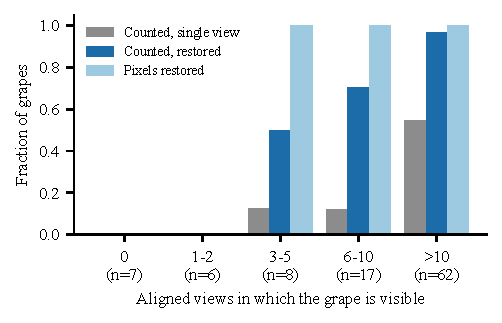
\includegraphics[width=0.9\linewidth]{figures/visibility.pdf}
\caption{Of the 100 labelled grapes (four captures, 20~mm), the fraction counted by GrapeSAM in the single view (grey) and in the reconstruction (dark blue, ``restored'' in the legend), and the fraction whose pixels the reconstruction recovered (light blue), by the number of aligned views in which each grape is visible. Grapes seen in at most two views are never recovered.}
\label{fig:visibility}
\end{figure}

\textbf{Runtime.} For five branches with 28 views at scale 0.8, on a laptop with an RTX~2000 Ada GPU, loading, matching and the joint solve took 16~s and fusion 209~s; SAM~3 masks took 1.5~s per view and GrapeSAM 0.6~s per image. Fusion, tiled NumPy code on the CPU, dominates, so the system currently suits offline analysis only.

\section{Discussion}
\textbf{Why count as well as pixels.} The two evaluations diverge: without colour consensus the reconstruction kept 89\% recall and 80\% precision yet count F1 fell from 0.77 to 0.26, and mask union matched our recall but lost 14--21 points of precision at three to five branches. A method tuned on pixel overlap alone could pick a configuration that looks better and counts worse, so counting goals need a count-based check.

\textbf{Comparison with related work.} Hemming \etal~\cite{hemming2014} found that combining viewpoints raised sweet pepper detectability from at most 69\% to 90\%. For our passive sweep at three to five branches, the share of grapes counted rose from 32--64\% to 80--96\% (labelled grapes matched by a detection, out of 25 per capture; the data of Fig.~\ref{fig:visibility}). The measures differ, so this is an analogy, not a ranking. Our baselines support replacing the assumed fruit depth of synthetic aperture imaging~\cite{vaish2006,kurmi2018} with fruit-only alignment. Learned corrections such as GCNet~\cite{quinones2025gcnet} and occlusion GANs~\cite{kierdorf2022} address what we cannot: fruit that no view saw. Every grape was visible in at least three aligned views at three to five branches, but 13 of 25 were visible in at most two at six branches. The approaches are therefore complementary: observation-backed recovery shrinks the hidden fraction before a learned or statistical correction~\cite{millan2018,nuske2014} is applied.

\textbf{Strengths and limitations.} The method needs one RGB camera and no depth sensor. Its reconstruction varied little across reference views (F1 standard deviation 0.04--0.05, against up to 0.18 for single views), and its gains exceeded the registration noise floor. Its limitations are as follows. All conditions share one arrangement of 25 grapes, so our intervals cover which grapes are present, the reference and the registration, but not variation between scenes. Fruit, foliage and truth masks all come from SAM~3, so GrapeSAM adds independence only at the counting stage. GrapeSAM was trained on field images~\cite{tong2026vivid} and overcounted even the leaf-free photograph. One similarity per view treats the fruit as a single plane, which contributes to cluster offsets and rejected views; the perturbation study bounds global registration error only, not this per-cluster offset, which is one reason the count metric is the primary result. Agreement is tested in raw RGB at a fixed threshold, so exposure or white-balance changes between views, or highlights that move with viewpoint, would reject true fruit; the rig held illumination constant. The joint solve, view validation, foliage mask and baseline rule had no effect at five branches, and their value where views fail is not shown. We tested occlusion (3--6 branches), spacing (20--60~mm), the number of views, the choice of reference and truth registration error. We did not test a second arrangement, green fruit, outdoor light, vehicle motion or yield.

\textbf{Future work.} The priority is repetition across arrangements, including green grapes, with held-out labels. Recovery under heavy occlusion was limited by alignment, so per-cluster or depth-aware alignment is the most promising change; our simulation-only depth-based variant (Sec.~\ref{sec:evolution}) suggests it is feasible but sensitive to pose error. A vehicle test in a vineyard row, with calibration against harvested mass, should follow.

\section{Conclusion}
In a controlled study, one RGB camera on a passive row-following sweep recovered hidden grapes by observation alone. At 20~mm spacing with five branches, fruit pixel recall rose from 42\% to 87\%, and the F1 of an independent counter rose from 0.42 to 0.77. Feature alignment outperformed depth-based synthetic aperture. Colour consensus kept the recovered fruit countable, an effect that pixel metrics alone missed. Recovery depended mainly on how many views passed alignment. Field use, green grapes and yield remain untested.

{
    \small
    \bibliographystyle{ieeenat_fullname}
    \bibliography{main}
}
\newpage
\section*{Statement of contributions}
% Each author checks their line before signing. Categories follow the handout:
% literature review, implementation, benchmark data, writing.
\noindent\textbf{Finn Panko-Jones.} Implementation: the rail rig and the four captures; the depth-shift synthetic aperture prototype; the final pipeline (fruit-only registration, joint pose solve and consensus fusion); the baselines, ablations and evaluation scripts. Writing: Secs.~\ref{sec:method} and 5.\\[2pt]
\textbf{Dinh Quang Huynh.} Implementation: SAM~3 fruit and foliage segmentation; red and green separation; the COLMAP background reconstruction. Benchmark data: the leaf-free photographs and the 25 grape labels. Writing: Sec.~\ref{sec:exp} and the figures.\\[2pt]
\textbf{Has Salvesen.} Literature review and Sec.~2. Implementation: a colour-free occlusion-aware synthetic aperture variant with its synthetic benchmark; the code repository and its documentation. Writing: abstract, introduction, discussion and conclusion; report integration and editing.\\[6pt]
\noindent Signed, 8 November 2026:\\[10pt]
\noindent Finn Panko-Jones \hrulefill\hspace{0.02\linewidth}\\[12pt]
\noindent Dinh Quang Huynh \hrulefill\hspace{0.02\linewidth}\\[12pt]
\noindent Has Salvesen \hrulefill\hspace{0.02\linewidth}

\section*{Acknowledgement of AI assistance}
ChatGPT (OpenAI) and Claude (Anthropic, including Claude Code) were used. ChatGPT assisted with structuring and drafting the LaTeX report, clarifying explanations of the method and checking citation and formatting consistency. Claude assisted with searching and summarising the literature, with writing and debugging code for the synthetic benchmark and the repository documentation, and with editing the text for clarity and consistency. All captures, experiments, measurements, figures and conclusions were produced, run and verified by the authors, who are responsible for the content.
% WARNING: do not forget to delete the supplementary pages from your submission 
% \input{sec/X_suppl}

\end{document}
